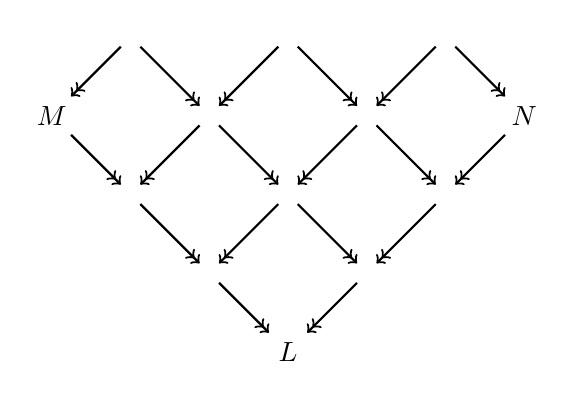
\begin{tikzpicture}[
    surj/.style={->>, line width=0.8pt},
    dashedsurj/.style={->>, dashed, line width=0.8pt}
    ]

    \node (K1) at (1,4) {};
    \node (K2) at (3,4) {};
    \node (K3) at (5,4) {};
    \node (M) at (0,3) {\(M\)};
    \node (K4) at (2,3) {};
    \node (K5) at (4,3) {};
    \node (N) at (6,3) {\(N\)};
    \node (K6) at (1,2) {};
    \node (K7) at (3,2) {};
    \node (K8) at (5,2) {};
    \node (K9) at (2,1) {};
    \node (K10) at (4,1) {};
    \node (L) at (3,0) {\(L\)};
    
    \draw[surj] (K1) -- (M);   \draw[surj] (K1) -- (K4);
    \draw[surj] (K2) -- (K4);  \draw[surj] (K2) -- (K5);
    \draw[surj] (K3) -- (K5);  \draw[surj] (K3) -- (N);
    \draw[surj] (M) -- (K6);
    \draw[surj] (N) -- (K8);
    \draw[surj] (K4) -- (K7);  \draw[surj] (K4) -- (K6);
    \draw[surj] (K5) -- (K7);  \draw[surj] (K5) -- (K8);
    \draw[surj] (K6) -- (K9);
    \draw[surj] (K7) -- (K9);  \draw[surj] (K7) -- (K10);
    \draw[surj] (K8) -- (K10);
    \draw[surj] (K9) -- (L);
    \draw[surj] (K10) -- (L);

\end{tikzpicture}